%%%%%%%%%%%%%%%%%%%%%%%%%%%%%%%%%%%%%%%%%
% Beamer Presentation
% LaTeX Template
% Version 1.0 (10/11/12)
%
% This template has been downloaded from:
% http://www.LaTeXTemplates.com
%
% License:
% CC BY-NC-SA 3.0 (http://creativecommons.org/licenses/by-nc-sa/3.0/)
%
%%%%%%%%%%%%%%%%%%%%%%%%%%%%%%%%%%%%%%%%%

%----------------------------------------------------------------------------------------
%	PACKAGES AND THEMES
%----------------------------------------------------------------------------------------

\documentclass{beamer}

\mode<presentation> {
\usetheme{Singapore}
\usecolortheme{rose}
\setbeamertemplate{footline}[page number]

\setbeamertemplate{navigation symbols}{} 
}

\usepackage{graphicx} % Allows including images
\usepackage{booktabs} % Allows the use of \toprule, \midrule and \bottomrule in tables
\usepackage{listings}
\usepackage{xcolor}
\usepackage{color}

\colorlet{punct}{red!60!black}
\definecolor{background}{HTML}{EEEEEE}
\definecolor{delim}{RGB}{25,134,57}
\colorlet{numb}{magenta!60!black}

\lstdefinelanguage{json}{
    basicstyle=\normalfont\ttfamily,
    numbers=left,
    numberstyle=\scriptsize,
    stepnumber=1,
    numbersep=8pt,
    showstringspaces=false,
    breaklines=true,
    frame=lines,
    backgroundcolor=\color{background},
    literate=
     *{0}{{{\color{numb}0}}}{1}
      {1}{{{\color{numb}1}}}{1}
      {2}{{{\color{numb}2}}}{1}
      {3}{{{\color{numb}3}}}{1}
      {4}{{{\color{numb}4}}}{1}
      {5}{{{\color{numb}5}}}{1}
      {6}{{{\color{numb}6}}}{1}
      {7}{{{\color{numb}7}}}{1}
      {8}{{{\color{numb}8}}}{1}
      {9}{{{\color{numb}9}}}{1}
      {:}{{{\color{punct}{:}}}}{1}
      {,}{{{\color{punct}{,}}}}{1}
      {\{}{{{\color{delim}{\{}}}}{1}
      {\}}{{{\color{delim}{\}}}}}{1}
      {[}{{{\color{delim}{[}}}}{1}
      {]}{{{\color{delim}{]}}}}{1},
}
%----------------------------------------------------------------------------------------
%	TITLE PAGE
%----------------------------------------------------------------------------------------

\title[AureliaJS]{AureliaJS} 
\author{Jesse Javier Cogollo Alvarez}
\institute[EAFIT - TalosDigital]
{
Developer by passion \\
\medskip
\textit{email: cogollo87@gmail.com} \\~\\
\textit{MedellinJS}
}
%\date{\today} % Date, can be changed to a custom date
\begin{document}

\begin{frame}
\titlepage % Print the title page as the first slide
\end{frame}

\begin{frame}
\frametitle{Contenido} % Table of contents slide, comment this block out to remove it
\tableofcontents % Throughout your presentation, if you choose to use \section{} and \subsection{} commands, these will automatically be printed on this slide as an overview of your presentation
\end{frame}

%----------------------------------------------------------------------------------------
%	PRESENTATION SLIDES
%----------------------------------------------------------------------------------------

%------------------------------------------------
\section{AureliaJS} % Sections can be created in order to organize your presentation into discrete blocks, all sections and subsections are automatically printed in the table of contents as an overview of the talk
%------------------------------------------------
\begin{frame}
\frametitle{Que es Aurelia?}
Aurelia is a next generation JavaScript client framework that leverages simple conventions to empower your creativity.
{\color{blue}\url{http://aurelia.io/}}
\\~\\
Rob Eisenberg

{\color{blue}\url{robeisenberg.com}}

%\begin{figure}
%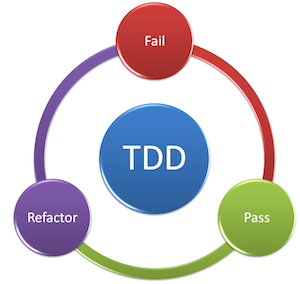
\includegraphics[width=0.3\linewidth]{tdd.png}
%\end{figure}
\end{frame}

%------------------------------------------------
\begin{frame}
\frametitle{Caracteristicas}
\begin{columns}[c] % The "c" option specifies centered vertical alignment while the "t" option is used for top vertical alignment

\column{.45\textwidth} % Left column and width
\begin{enumerate}
\item \textbf{Forward-thinking}
\item[•]	
\item[•]	
\item[•]	
\item[•]	
\item[•]	
\item[•]	
\item[•]	
\end{enumerate}

\column{.5\textwidth} % Right column and width
Escrito con ES6 y ES7. se integra con web components. no tiene dependencias externas (excepto polyfills).
\end{columns}
\end{frame}

%------------------------------------------------

\begin{frame}
\frametitle{Caracteristicas}
\begin{columns}[c] % The "c" option specifies centered vertical alignment while the "t" option is used for top vertical alignment

\column{.45\textwidth} % Left column and width
\begin{enumerate}
\item \textbf{Forward-thinking}
\item \textbf{Modern Architecture}
\item[•]	
\item[•]	
\item[•]	
\item[•]	
\item[•]	
\item[•]	
\end{enumerate}

\column{.5\textwidth} % Right column and width
Aurelia esta compuesto por pequenos modulos. Utiliados juntos como un completo framework. Pero tambien permite personalizarlo con diferentes modulos.
\end{columns}
\end{frame}

%------------------------------------------------
\begin{frame}
\frametitle{Caracteristicas}
\begin{columns}[c] % The "c" option specifies centered vertical alignment while the "t" option is used for top vertical alignment

\column{.45\textwidth} % Left column and width
\begin{enumerate}
\item \textbf{Forward-thinking}
\item \textbf{Modern Architecture}
\item \textbf{Two-Way Databinding}
\item[•]	
\item[•]	
\item[•]	
\item[•]	
\item[•]	
\end{enumerate}

\column{.5\textwidth} % Right column and width
Aurelia tiene una poderosa two-way binding. el cual utiliza tecnicas adaptativas para utilizar el mecanismo mas eficiente para observar cada propiedad. Object.observer
\end{columns}
\end{frame}

%------------------------------------------------
\begin{frame}
\frametitle{Caracteristicas}
\begin{columns}[c] % The "c" option specifies centered vertical alignment while the "t" option is used for top vertical alignment

\column{.45\textwidth} % Left column and width
\begin{enumerate}
\item \textbf{Forward-thinking}
\item \textbf{Modern Architecture}
\item \textbf{Two-Way Databinding}
\item \textbf{Extensible HTML}
\item[•]	
\item[•]	
\item[•]	
\item[•]	
\end{enumerate}

\column{.5\textwidth} % Right column and width
La extensibilidad HTML de Aurelia permite crear elementos HTML personalizados, anadir nuevos comportamientos para elementos ya existentes.
\end{columns}
\end{frame}

%------------------------------------------------
\begin{frame}
\frametitle{Caracteristicas}
\begin{columns}[c] % The "c" option specifies centered vertical alignment while the "t" option is used for top vertical alignment

\column{.45\textwidth} % Left column and width
\begin{enumerate}
\item \textbf{Forward-thinking}
\item \textbf{Modern Architecture}
\item \textbf{Two-Way Databinding}
\item \textbf{Extensible HTML}
\item \textbf{Routing and UI Composition}
\item[•]	
\item[•]	
\item[•]	
\end{enumerate}

\column{.5\textwidth} % Right column and width
Router con acoplamiento activo, patrones de ruta dinamica, activacion de pantallas asincronicamente, etc.
\end{columns}
\end{frame}

%------------------------------------------------
\begin{frame}
\frametitle{Caracteristicas}
\begin{columns}[c] % The "c" option specifies centered vertical alignment while the "t" option is used for top vertical alignment

\column{.45\textwidth} % Left column and width
\begin{enumerate}
\item \textbf{Forward-thinking}
\item \textbf{Modern Architecture}
\item \textbf{Two-Way Databinding}
\item \textbf{Extensible HTML}
\item \textbf{Routing and UI Composition}
\item \textbf{MV* with Conventions}
\item[•]	
\item[•]	
\end{enumerate}

\column{.5\textwidth} % Right column and width
Quieres invertir tiempo en escribir codigo de configuracion? Aurelia maneja una convecion simple.
\end{columns}
\end{frame}

%------------------------------------------------

%------------------------------------------------
\begin{frame}
\frametitle{Caracteristicas}
\begin{columns}[c] % The "c" option specifies centered vertical alignment while the "t" option is used for top vertical alignment

\column{.45\textwidth} % Left column and width
\begin{enumerate}
\item \textbf{Forward-thinking}
\item \textbf{Modern Architecture}
\item \textbf{Two-Way Databinding}
\item \textbf{Extensible HTML}
\item \textbf{Routing and UI Composition}
\item \textbf{MV* with Conventions}
\item \textbf{Broad Language Support}
\item[•]	
\end{enumerate}

\column{.5\textwidth} % Right column and width
Utiliza ES5, ES6, TypeScript, AtScript, CoffeeScript.
\end{columns}
\end{frame}

%------------------------------------------------

%------------------------------------------------
\begin{frame}
\frametitle{Caracteristicas}
\begin{columns}[c] % The "c" option specifies centered vertical alignment while the "t" option is used for top vertical alignment

\column{.45\textwidth} % Left column and width
\begin{enumerate}
\item \textbf{Forward-thinking}
\item \textbf{Modern Architecture}
\item \textbf{Two-Way Databinding}
\item \textbf{Extensible HTML}
\item \textbf{Routing and UI Composition}
\item \textbf{MV* with Conventions}
\item \textbf{Broad Language Support}
\item \textbf{Testable}
\end{enumerate}

\column{.5\textwidth} % Right column and width
combinando modulos ES6 con contenedor inyeccion de dependencias. se hace mas facil crear codigo altamente cohesivo y bajo acoplamiento. haciendo las pruebas unitarias algo facil.
\end{columns}
\end{frame}

%------------------------------------------------

\begin{frame}
\frametitle{Como empezar - Estructura}
Descargamos la ultima version del skeleton de aurelia.
\\~\\
{\color{blue}\url{https://github.com/aurelia/skeleton-navigation/releases/tag/0.15.1}}
\\~\\
descomprimimos y ya tenemos una estrutura lista para utilizar:
\begin{itemize}
\item build (configuracion gulp).
\item doc (documentacion).
\item src (codificacion).
\item styles (estilos CSS).
\item test (pruebas).
\item README.md (instrucciones para utilizar AureliaJS).
\end{itemize}
\end{frame}

%------------------------------------------------

%------------------------------------------------

%\begin{frame}
%\frametitle{Como empezar}
%Descargamos la ultima version del skeleton de aurelia.
%\begin{itemize}
%\item No utilizan el modelo relacional.
%\item Corren bien en clusters.
%\item Open-source.
%\item sin esquemas.
%\item El resultado mas importante del aumento de las bases de datos NoSQL es la {\color{green}Persistencia %Poliglota}.
%\end{itemize}
%{\color{blue}\url{Descargar: https://github.com/aurelia/skeleton-navigation/releases/tag/0.15.1}}
%\end{frame}

%------------------------------------------------

%------------------------------------------------
\begin{frame}
\frametitle{Modulos}
\begin{columns}[c] % The "c" option specifies centered vertical alignment while the "t" option is used for top vertical alignment

\column{.45\textwidth} % Left column and width
\begin{itemize}
\item \textbf{logging}
\end{itemize}

\column{.5\textwidth} % Right column and width
Esta libreria es parte de la plataforma aurelia y contiene un "Appender" para el logging.
\\~\\
uso:
\\~\\
import {computedFrom, LogManager} from 'aurelia-framework';
\\~\\
var logger = LogManager.getLogger('mi log');
\\~\\
logger.info('log info');
\end{columns}
\end{frame}

%------------------------------------------------
\begin{frame}
\frametitle{Modulos}
\begin{columns}[c] % The "c" option specifies centered vertical alignment while the "t" option is used for top vertical alignment

\column{.45\textwidth} % Left column and width
\begin{itemize}
\item \textbf{Plugins}
\end{itemize}

\column{.5\textwidth} % Right column and width
Aurelia permite crear e implementar plugins que se adaptan a Aurelia.
Estos plugins se configuran en:
\\~\\ <body aurelia-app="namefile">
\end{columns}
\end{frame}

%------------------------------------------------
\begin{frame}
\frametitle{Caracteristicas}
\begin{columns}[c] % The "c" option specifies centered vertical alignment while the "t" option is used for top vertical alignment

\column{.45\textwidth} % Left column and width
\begin{itemize}
\item \textbf{Aurelia Object}
\end{itemize}

\column{.5\textwidth} % Right column and width
Aurelia Object (TODO)
\end{columns}
\end{frame}

%------------------------------------------------
\begin{frame}
\frametitle{Vistas y vistas modelos}
\begin{columns}[c] % The "c" option specifies centered vertical alignment while the "t" option is used for top vertical alignment

\column{.45\textwidth} % Left column and width
\begin{itemize}
\item \textbf{DI inyeccion de dependencias}
\end{itemize}

\column{.5\textwidth} % Right column and width
DI inyeccion de dependencias (TODO)
\end{columns}
\end{frame}

%------------------------------------------------
\begin{frame}
\frametitle{Vistas y vistas modelos}
\begin{columns}[c] % The "c" option specifies centered vertical alignment while the "t" option is used for top vertical alignment

\column{.45\textwidth} % Left column and width
\begin{itemize}
\item \textbf{Modelos de vista padre}
\end{itemize}

\column{.5\textwidth} % Right column and width
Modelos de vista padre (TODO)
\end{columns}
\end{frame}

%------------------------------------------------
\begin{frame}
\frametitle{Vistas y vistas modelos}
\begin{columns}[c] % The "c" option specifies centered vertical alignment while the "t" option is used for top vertical alignment

\column{.45\textwidth} % Left column and width
\begin{itemize}
\item \textbf{Plantillas}
\end{itemize}

\column{.5\textwidth} % Right column and width
Plantillas (TODO)
\end{columns}
\end{frame}

\section{DEMO}
%------------------------------------------------
\begin{frame}
\frametitle{Databiding}
\begin{columns}[c] % The "c" option specifies centered vertical alignment while the "t" option is used for top vertical alignment

\column{.45\textwidth} % Left column and width
\begin{itemize}
\item \textbf{Que es}
\end{itemize}

\column{.5\textwidth} % Right column and width
Databiding (TODO)
\end{columns}
\end{frame}
%------------------------------------------------

\begin{frame}
\frametitle{Coding Dojo}
\begin{columns}[c] % The "c" option specifies centered vertical alignment while the "t" option is used for top vertical alignment

\column{.45\textwidth} % Left column and width
\begin{enumerate}
\item \textbf{Que es}
\item \textbf{estilo 1}
\item[•]
\item[•]
\item[•]

\end{enumerate}

\column{.5\textwidth} % Right column and width
\textbf{randori} Muchos programadores un problema.
\end{columns}
\end{frame}
%------------------------------------------------

\begin{frame}
\frametitle{Coding Dojo}
\begin{columns}[c] % The "c" option specifies centered vertical alignment while the "t" option is used for top vertical alignment

\column{.45\textwidth} % Left column and width
\begin{enumerate}
\item \textbf{Que es}
\item \textbf{estilo 1}
\item \textbf{estilo 2}
\item[•]
\item[•]

\end{enumerate}

\column{.5\textwidth} % Right column and width
Pair programming en paralelo. (Cyberdojo.org)
\end{columns}
\end{frame}
%------------------------------------------------

\begin{frame}
\frametitle{Coding Dojo}
\begin{columns}[c] % The "c" option specifies centered vertical alignment while the "t" option is used for top vertical alignment

\column{.45\textwidth} % Left column and width
\begin{enumerate}
\item \textbf{Que es}
\item \textbf{estilo 1}
\item \textbf{estilo 2}
\item \textbf{estilo 3}
\item[•]

\end{enumerate}

\column{.5\textwidth} % Right column and width
Trabajando bajo presi\'on. (Extreme startup)
\end{columns}
\end{frame}
%------------------------------------------------

\begin{frame}
\frametitle{Coding Dojo}
\begin{columns}[c] % The "c" option specifies centered vertical alignment while the "t" option is used for top vertical alignment

\column{.45\textwidth} % Left column and width
\begin{enumerate}
\item \textbf{Que es}
\item \textbf{estilo 1}
\item \textbf{estilo 2}
\item \textbf{estilo 3}
\item \textbf{recursos}
\end{enumerate}

\column{.5\textwidth} % Right column and width
\begin{itemize}
\item Un computador con el ambiente de desarrollo listo. 
\item un projector 
\item un lugar para runirse
\item un facilitador
\item entre 4 y muchos programadores con ganas de divertirse.
\end{itemize}
\end{columns}
\end{frame}
%------------------------------------------------
\begin{frame}
\frametitle{Redes sociales}
\begin{columns}[c] % The "c" option specifies centered vertical alignment while the "t" option is used for top vertical alignment

\column{.45\textwidth} % Left column and width
\begin{enumerate}
\item \textbf{Meetup}
\item[•]	
\item[•]	
\item[•]	
\item[•]	
\end{enumerate}

\column{.5\textwidth} % Right column and width
%\begin{figure}
%
\includegraphics[width=0.5\linewidth]{meetup.png}
%\end{figure}
{\color{blue}/MongoDB-Medellin}
\\~\\
{\color{blue}\url{http://goo.gl/fw5Gyh}}
\end{columns}
\end{frame}
%------------------------------------------------

\begin{frame}
\frametitle{Redes sociales}
\begin{columns}[c] % The "c" option specifies centered vertical alignment while the "t" option is used for top vertical alignment

\column{.45\textwidth} % Left column and width
\begin{enumerate}
\item Meetup
\item \textbf{Twitter}
\item[•]	
\item[•]	
\item[•]	
\end{enumerate}

\column{.5\textwidth} % Right column and width
%\begin{figure}
%
\includegraphics[width=0.5\linewidth]{twitter.png}
%\end{figure}
{\color{blue}@jessecogollo}
\\~\\
{\color{blue}\url{http://goo.gl/gdCAjF}}
\end{columns}
\end{frame}
%------------------------------------------------

\begin{frame}
\frametitle{Redes sociales}
\begin{columns}[c] % The "c" option specifies centered vertical alignment while the "t" option is used for top vertical alignment

\column{.45\textwidth} % Left column and width
\begin{enumerate}
\item Meetup
\item Twitter
\item \textbf{Facebook}
\item[•]	
\item[•]	
\end{enumerate}

\column{.5\textwidth} % Right column and width
%\begin{figure}
%
\includegraphics[width=0.5\linewidth]{facebook.png}
%\end{figure}
{\color{blue}/jessecogollo}
\\~\\
{\color{blue}\url{http://goo.gl/Q1JnXQ}}
\end{columns}
\end{frame}
%------------------------------------------------	
\begin{frame}
\frametitle{Redes sociales}
\begin{columns}[c] % The "c" option specifies centered vertical alignment while the "t" option is used for top vertical alignment

\column{.45\textwidth} % Left column and width
\begin{enumerate}
\item Meetup
\item Twitter
\item Facebook
\item Google Plus
\item \textbf{Lista de correo}
\item[•]	
\end{enumerate}

\column{.5\textwidth} % Right column and width
%\begin{figure}
%
\includegraphics[width=0.5\linewidth]{gmail.png}
%\end{figure}
{\color{blue}+ correo}
\\~\\
{\color{blue}\url{http://goo.gl/FJvrjT}}
\end{columns}
\end{frame}
%------------------------------------------------	
\begin{frame}
\frametitle{Redes sociales}
\begin{columns}[c] % The "c" option specifies centered vertical alignment while the "t" option is used for top vertical alignment

\column{.45\textwidth} % Left column and width
\begin{enumerate}
\item Meetup
\item Twitter
\item Facebook
\item Google Plus
\item Lista de correo
\item \textbf{Grupo de estudio}
\end{enumerate}

\column{.5\textwidth} % Right column and width
%\begin{figure}
%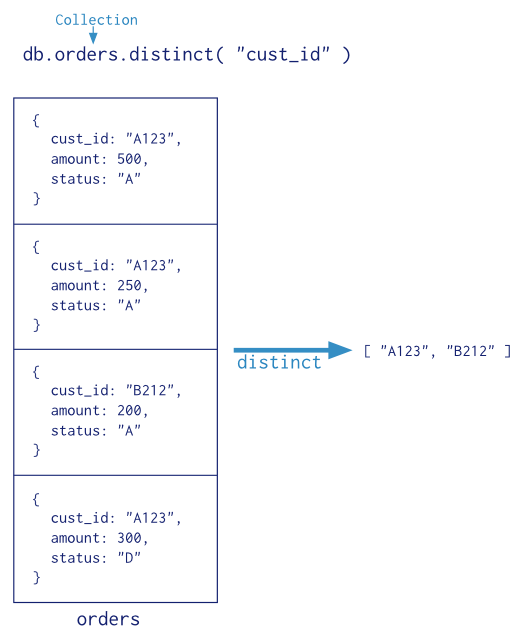
\includegraphics[width=0.5\linewidth]{distinct.png}
%\end{figure}
{\color{blue}Formulario grupo de estudio}
\\~\\
{\color{blue}\url{http://goo.gl/7ALdst}}
\end{columns}
\end{frame}
%------------------------------------------------	
\begin{frame}
\frametitle{Donde aprender}
\begin{columns}[c] % The "c" option specifies centered vertical alignment while the "t" option is used for top vertical alignment
\column{.45\textwidth} % Left column and width
\begin{enumerate}
\item \textbf{Organizar un coding dojo}
\item[•]
\item[•]
\item[•]
\item[•]
\end{enumerate}

\column{.5\textwidth} % Right column and width
%\begin{figure}
%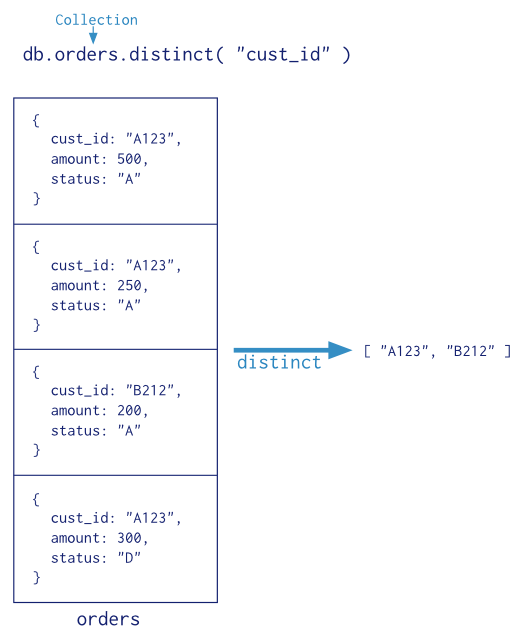
\includegraphics[width=0.5\linewidth]{distinct.png}
%\end{figure}
{\color{blue}\url{http://johannesbrodwall.com/2011/12/18/how-to-start-a-coding-dojo/}}
\end{columns}
\end{frame}
%------------------------------------------------	
\begin{frame}
\frametitle{Donde aprender}
\begin{columns}[c] % The "c" option specifies centered vertical alignment while the "t" option is used for top vertical alignment
\column{.45\textwidth} % Left column and width
\begin{enumerate}
\item Organizar un coding dojo
\item \textbf{Cyber dojo}
\item[•]
\item[•]
\item[•]
\end{enumerate}

\column{.5\textwidth} % Right column and width
%\begin{figure}
%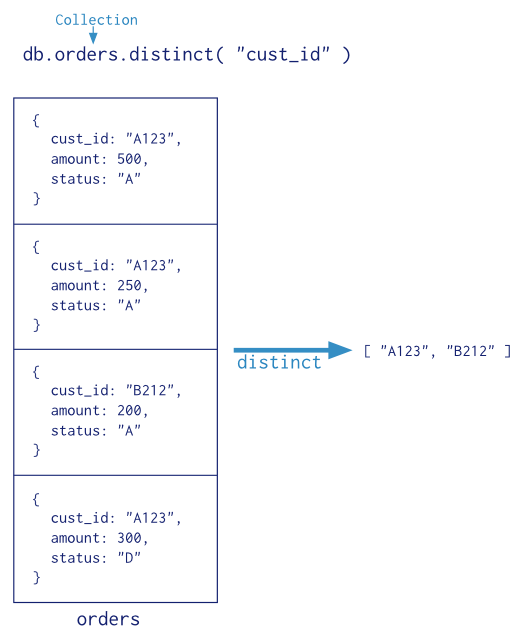
\includegraphics[width=0.5\linewidth]{distinct.png}
%\end{figure}
{\color{blue}\url{http://cyber-dojo.org/}}
\end{columns}
\end{frame}
%------------------------------------------------	
\begin{frame}
\frametitle{Donde aprender}
\begin{columns}[c] % The "c" option specifies centered vertical alignment while the "t" option is used for top vertical alignment
\column{.45\textwidth} % Left column and width
\begin{enumerate}
\item Organizar un coding dojo
\item Cyber dojo
\item \textbf{Codingdojo}
\item[•]
\item[•]
\end{enumerate}

\column{.5\textwidth} % Right column and width
%\begin{figure}
%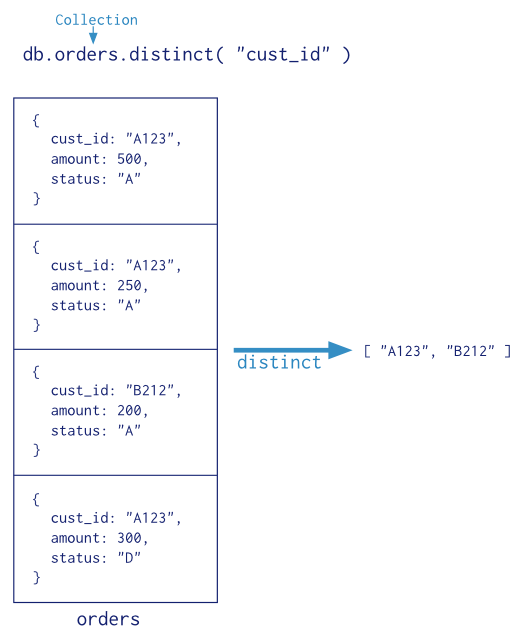
\includegraphics[width=0.5\linewidth]{distinct.png}
%\end{figure}
{\color{blue}\url{http://www.codingdojo.org/}}
\end{columns}
\end{frame}
%------------------------------------------------	
\begin{frame}
\frametitle{Donde aprender}
\begin{columns}[c] % The "c" option specifies centered vertical alignment while the "t" option is used for top vertical alignment
\column{.45\textwidth} % Left column and width
\begin{enumerate}
\item Organizar un coding dojo
\item Cyber dojo
\item Codingdojo
\item \textbf{Ejercicios}
\item[•]
\end{enumerate}

\column{.5\textwidth} % Right column and width
%\begin{figure}
%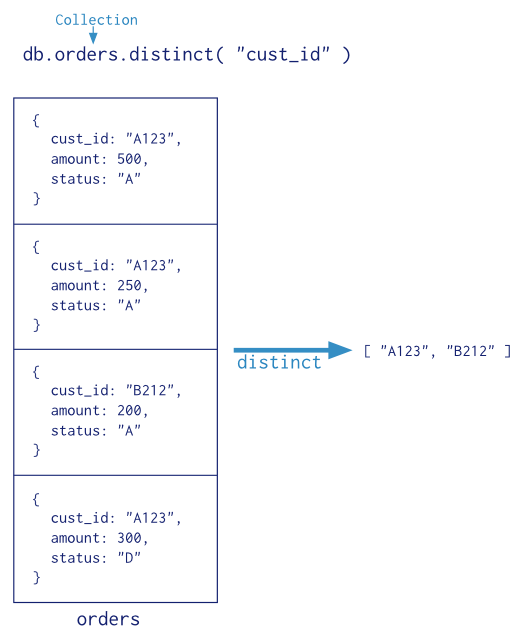
\includegraphics[width=0.5\linewidth]{distinct.png}
%\end{figure}
{\color{blue}\url{http://rosettacode.org/wiki/Category:Programming_Tasks}}
\end{columns}
\end{frame}
%------------------------------------------------	
\begin{frame}
\frametitle{Donde aprender}
\begin{columns}[c] % The "c" option specifies centered vertical alignment while the "t" option is used for top vertical alignment
\column{.45\textwidth} % Left column and width
\begin{enumerate}
\item Organizar un coding dojo
\item Cyber dojo
\item Codingdojo
\item Ejercicios
\item \textbf{Mas ejercicios}
\end{enumerate}

\column{.5\textwidth} % Right column and width
%\begin{figure}
%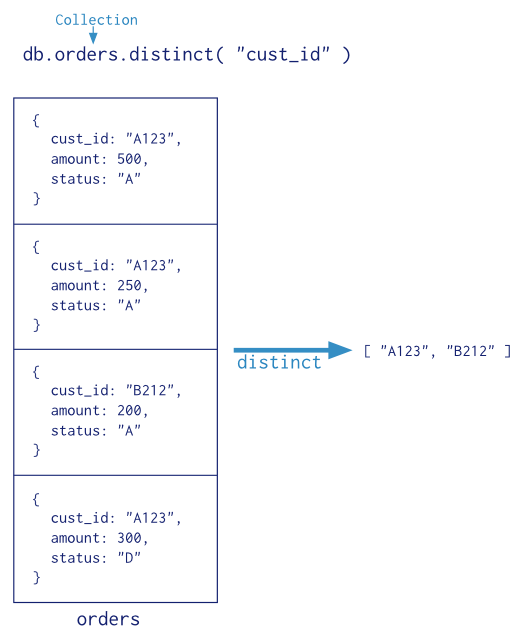
\includegraphics[width=0.5\linewidth]{distinct.png}
%\end{figure}
{\color{blue}\url{http://brendan.enrick.com/post/Coding-Katas-and-Exercises}}
\end{columns}
\end{frame}
%------------------------------------------------
\begin{frame}
\frametitle{Preguntas}
%\begin{figure}
%
\includegraphics[width=0.4\linewidth]{preguntas.png}
%\end{figure}
\end{frame}
%------------------------------------------------
\begin{frame}
\frametitle{Empecemos...}
\begin{figure}
%
\includegraphics[width=0.4\linewidth]{happy.png}
\end{figure}
\end{frame}
%------------------------------------------------
\begin{frame}
\Huge{\centerline{Gracias !!! =)}}
\end{frame}

%----------------------------------------------------------------------------------------

\end{document} 
